% !TeX program = xelatex
% !TeX root = text.tex
\documentclass[a4paper,12pt]{ctexart}

% 导入必要的包
\usepackage{geometry}  % 页面设置
\usepackage{titlesec}  % 标题格式
\usepackage{fancyhdr}  % 页眉页脚
\usepackage{setspace}  % 行距设置
\usepackage{enumitem}  % 列表环境
\usepackage{graphicx}  % 图片支持
\usepackage{hyperref}  % 超链接
\usepackage{indentfirst}  % 首行缩进
\usepackage{xeCJK}  % 中文字体支持
\usepackage{tabularx}  % 表格支持
\usepackage{booktabs}  % 表格线
\usepackage{multirow}  % 表格合并单元格
\usepackage{tocloft}  % 目录格式设置
\hypersetup{pageanchor=false}  % 解决页码标签问题
\setmainfont{Times New Roman}  % 英文和数字
\usepackage{cite}  % 添加引用包
\DeclareGraphicsExtensions{.png,.pdf,.jpg}
\graphicspath{{figures/}}  % 设置图片搜索路径

% 在导言区添加字体映射设置
\defaultfontfeatures{Mapping=tex-text}

% 设置中文字体
\setCJKmainfont[BoldFont={SimHei}]{SimSun}
\setCJKsansfont[BoldFont={SimHei}]{Microsoft YaHei}
\setCJKmonofont[BoldFont={SimHei}]{FangSong}

% 字体设置(修改为更合适的设置)
\setCJKfamilyfont{zhsong}[BoldFont={SimHei}]{SimSun}
\setCJKfamilyfont{zhhei}[BoldFont={SimHei}]{SimHei}
\setCJKfamilyfont{zhkai}[BoldFont={SimHei}]{KaiTi}
\newcommand{\song}{\CJKfamily{zhsong}}
\newcommand{\hei}{\CJKfamily{zhhei}}
\newcommand{\kai}{\CJKfamily{zhkai}}

% 定义字体大小
\newcommand{\yihao}{\fontsize{26pt}{39pt}\selectfont}      % 1号
\newcommand{\xiaochu}{\fontsize{36pt}{54pt}\selectfont}    % 小初
\newcommand{\sanhao}{\fontsize{16pt}{24pt}\selectfont}     % 3号
\newcommand{\sihao}{\fontsize{14pt}{21pt}\selectfont}      % 4号
\newcommand{\xiaosihao}{\fontsize{12pt}{18pt}\selectfont}  % 小4号
\newcommand{\wuhao}{\fontsize{10.5pt}{15.75pt}\selectfont} % 5号
\newcommand{\xiaowuhao}{\fontsize{9pt}{13.5pt}\selectfont} % 小5号

% 页面设置
\geometry{
    left=3.18cm,
    right=3.18cm,
    top=2.54cm,
    bottom=2.54cm
}

% 设置行距为1.25倍
\setstretch{1.25}

% 设置段落格式
\setlength{\parindent}{2em}  % 首行缩进2字符
\setlength{\parskip}{0pt}    % 段落间距为0
\setlength{\baselineskip}{1.25\baselineskip}  % 行距为1.25倍

% 设置章节编号格式
\renewcommand{\thesection}{第\chinese{section}章}
\renewcommand{\thesubsection}{\arabic{section}.\arabic{subsection}}
\renewcommand{\thesubsubsection}{\arabic{section}.\arabic{subsection}.\arabic{subsubsection}}

% 设置标题格式
\titleformat{\section}{\centering\songti\sanhao\bfseries}{\thesection}{1em}{}
\titleformat{\subsection}{\songti\xiaosihao\bfseries}{\thesubsection}{1em}{}
\titleformat{\subsubsection}{\songti\wuhao\bfseries}{\thesubsubsection}{1em}{}

% 设置标题间距
\titlespacing{\section}{0pt}{24pt}{18pt}
\titlespacing{\subsection}{0pt}{12pt}{6pt}
\titlespacing{\subsubsection}{2em}{12pt}{6pt}

% 设置页眉页脚
\pagestyle{fancy}
\fancyhf{}
\fancyfoot[C]{\thepage}
\renewcommand{\headrulewidth}{0pt}

% 设置页码字体
\renewcommand{\thepage}{\songti\xiaowuhao\arabic{page}}

% 设置前文页码格式(罗马数字)
\pagenumbering{Roman}
\setcounter{page}{1}

% 设置正文页码格式(阿拉伯数字)
\newcommand{\startmainmatter}{
    \clearpage
    \pagenumbering{arabic}
    \setcounter{page}{1}
}

% 设置行距
\setstretch{1.5}  % 1.5倍行距
\setlength{\baselineskip}{18pt}  % 最小值18磅

% 设置目录格式
\renewcommand{\contentsname}{\centering\songti\sanhao\bfseries 目\quad 录}

% 设置章节编号格式
\renewcommand{\thesection}{第\chinese{section}章}
\renewcommand{\thesubsection}{\arabic{section}.\arabic{subsection}}
\renewcommand{\thesubsubsection}{\arabic{section}.\arabic{subsection}.\arabic{subsubsection}}

% 设置标题格式
\titleformat{\section}{\centering\songti\sanhao\bfseries}{\thesection}{1em}{}
\titleformat{\subsection}{\songti\xiaosihao\bfseries}{\thesubsection}{1em}{}
\titleformat{\subsubsection}{\songti\wuhao\bfseries}{\thesubsubsection}{1em}{}

% 设置标题间距
\titlespacing{\section}{0pt}{24pt}{18pt}
\titlespacing{\subsection}{0pt}{12pt}{6pt}
\titlespacing{\subsubsection}{2em}{12pt}{6pt}

% 设置目录格式
\renewcommand{\cftsecfont}{\songti\xiaosihao\bfseries}
\renewcommand{\cftsubsecfont}{\songti\wuhao}
\renewcommand{\cftsubsubsecfont}{\songti\wuhao}
\renewcommand{\cftsecpagefont}{\songti\xiaowuhao}
\renewcommand{\cftsubsecpagefont}{\songti\xiaowuhao}
\renewcommand{\cftsubsubsecpagefont}{\songti\xiaowuhao}

% 设置目录点线
\renewcommand{\cftsecleader}{\cftdotfill{\cftdotsep}}
\renewcommand{\cftsubsecleader}{\cftdotfill{\cftdotsep}}
\renewcommand{\cftsubsubsecleader}{\cftdotfill{\cftdotsep}}

% 设置目录缩进
\setlength{\cftsubsecindent}{2em}
\setlength{\cftsubsubsecindent}{4em}

% 设置目录深度
\setcounter{tocdepth}{3}
\setcounter{secnumdepth}{3}

% 自定义字体族
\setCJKfamilyfont{zhsong}[BoldFont={SimHei}]{SimSun}
\setCJKfamilyfont{zhhei}[BoldFont={SimHei}]{SimHei}
\setCJKfamilyfont{zhkai}[BoldFont={SimHei}]{KaiTi}

% 修改目录格式,避免hyperref警告
\renewcommand{\cftsecpresnum}{\hspace{0pt}}
\renewcommand{\cftsubsecpresnum}{\hspace{0pt}}
\renewcommand{\cftsubsubsecpresnum}{\hspace{0pt}}

% 设置摘要环境
\newenvironment{cnabstract}{
    \clearpage
    \thispagestyle{empty}
    \begin{center}
        \heiti\sanhao\bfseries 摘\quad 要
    \end{center}
    \vspace{2em}
    \songti\wuhao\par
}

% 设置英文摘要环境
\newenvironment{enabstract}{
    \clearpage
    \thispagestyle{empty}
    \begin{center}
        \bfseries\Large Abstract
    \end{center}
    \vspace{2em}
    \normalsize\par
}

% 设置目录格式
\renewcommand{\contentsname}{\centering\heiti\sanhao\bfseries 目\quad 录}

% 设置附件格式
\newcommand{\appendixitem}[2]{
    \noindent\songti\xiaosihao\bfseries 附件#1:#2\hfill 共\hspace{1em}\underline{\hspace{2em}}页
}

% 调整表格设置
\setlength{\tabcolsep}{3pt}  % 进一步减小表格列间距
\renewcommand{\arraystretch}{1.1}  % 稍微调整行距

% 设置三级标题下的列表格式
\newenvironment{subpoints}{
    \begin{enumerate}[label=(\arabic*),leftmargin=2em,itemsep=0pt,parsep=0pt]
    \songti\wuhao
}{
    \end{enumerate}
}

\begin{document}

% 封面页
\begin{titlepage}
    \centering
    \vspace*{2cm}
    
    % 学校名称(楷体1号)
    {\yihao\kaishu 北京信息科技大学}\\[3cm]
    
    % 论文类型(楷体小初加粗)
    {\xiaochu\kaishu\bfseries 毕业设计(论文)}\\[4cm]
    
    % 论文题目(宋体4号)
    {\sihao\songti
    题\quad 目:\underline{\hspace{8cm}}\\[1cm]
    
    学\quad 院:\underline{\hspace{8cm}}\\[1cm]
    
    专\quad 业:\underline{\hspace{8cm}}\\[1cm]
    
    学生姓名:\underline{\hspace{4cm}}班级/学号:\underline{\hspace{4cm}}\\[1cm]
    
    指导老师/督导老师:\underline{\hspace{8cm}}\\[1cm]
    
    起止时间:\underline{\hspace{2cm}}年\underline{\hspace{2cm}}月\underline{\hspace{2cm}}日 至 
    \underline{\hspace{2cm}}年\underline{\hspace{2cm}}月\underline{\hspace{2cm}}日
    }
    
    \vfill
\end{titlepage}

% 任务书与声明
\section*{毕业设计(论文)任务书}
\thispagestyle{empty}
\begin{center}
    \heiti\sanhao\bfseries 毕业设计(论文)任务书
\end{center}
\vspace{2em}

\begin{tabularx}{\textwidth}{|X|X|}
    \hline
    \multicolumn{2}{|c|}{\heiti\sihao 基本信息} \\
    \hline
    学生姓名 & \underline{\hspace{6cm}} \\
    \hline
    学号 & \underline{\hspace{6cm}} \\
    \hline
    专业 & \underline{\hspace{6cm}} \\
    \hline
    指导教师 & \underline{\hspace{6cm}} \\
    \hline
    题目 & \underline{\hspace{6cm}} \\
    \hline
\end{tabularx}
\vspace{2em}

\begin{tabularx}{\textwidth}{|X|}
    \hline
    \multicolumn{1}{|c|}{\heiti\sihao 任务内容} \\
    \hline
    \songti\wuhao
    1. 研究背景与意义:\underline{\hspace{0.8\textwidth}} \\
    \hline
    2. 主要研究内容:\underline{\hspace{0.8\textwidth}} \\
    \hline
    3. 预期目标:\underline{\hspace{0.8\textwidth}} \\
    \hline
    4. 进度安排:\underline{\hspace{0.8\textwidth}} \\
    \hline
\end{tabularx}
\vspace{2em}

\begin{tabularx}{\textwidth}{|X|X|}
    \hline
    \multicolumn{2}{|c|}{\heiti\sihao 指导教师意见} \\
    \hline
    签名: & 日期:\underline{\hspace{4cm}} \\
    \hline
\end{tabularx}
\vspace{2em}

\begin{tabularx}{\textwidth}{|X|X|}
    \hline
    \multicolumn{2}{|c|}{\heiti\sihao 系(教研室)意见} \\
    \hline
    签名: & 日期:\underline{\hspace{4cm}} \\
    \hline
\end{tabularx}

\clearpage

% 原创性声明
\section*{原创性声明}
\thispagestyle{empty}
\begin{center}
    \heiti\sanhao\bfseries 原创性声明
\end{center}
\vspace{2em}

\songti\wuhao
本人郑重声明:所呈交的毕业设计(论文)是本人在导师指导下进行的研究工作及取得的研究成果。尽我所知,除了文中特别加以标注和致谢的地方外,论文中不包含其他人已经发表或撰写过的研究成果。与我一同工作的同志对本研究所做的贡献均已在论文中作了明确的说明。

\vspace{4em}
\begin{tabularx}{\textwidth}{|X|X|}
    \hline
    作者签名:\underline{\hspace{4cm}} & 日期:\underline{\hspace{4cm}} \\
    \hline
\end{tabularx}

\clearpage

% 版权授权声明
\section*{版权授权声明}
\thispagestyle{empty}
\begin{center}
    \heiti\sanhao\bfseries 版权授权声明
\end{center}
\vspace{2em}

\songti\wuhao
本人完全了解北京信息科技大学有关保留、使用学位论文的规定,即:学校有权保留送交论文的复印件,允许论文被查阅和借阅;学校可以公布论文的全部或部分内容,可以采用影印、缩印或其他复制手段保存论文。

\vspace{4em}
\begin{tabularx}{\textwidth}{|X|X|}
    \hline
    作者签名:\underline{\hspace{4cm}} & 日期:\underline{\hspace{4cm}} \\
    \hline
    导师签名:\underline{\hspace{4cm}} & 日期:\underline{\hspace{4cm}} \\
    \hline
\end{tabularx}

\clearpage

% 中文摘要
\begin{cnabstract}
随着互联网信息的爆炸式增长,特别是以微信公众号为代表的自媒体平台的兴起,用户面临海量信息的获取和管理挑战。本研究的目的是设计并实现一个能够高效、智能地面向微信公众号进行信息采集、管理、检索与分析的系统,旨在为用户提供便捷的微信公众号信息获取与管理工具,提升信息利用效率。在方法上,系统采用现代化的前后端分离架构;后端基于Spring Boot框架,整合WebMagic实现微信文章的自动化爬取、内容解析和图片本地化存储,利用Apache Lucene构建高性能的全文索引,实现快速检索。系统集成了DeepSeek AI模型,以实现文章的智能摘要生成和关键词提取功能,并通过TF-IDF算法优化标签系统。前端则基于Vue.js和Element Plus构建用户友好且响应式的交互界面。经过测试,开发的系统具备微信公众号文章的采集、结构化存储、多维度检索、AI辅助内容分析及标签化管理等功能,成果表明系统运行稳定,各项功能达到了预期目标。本系统的意义在于为个人用户及研究者提供高效的微信公众号信息获取与管理工具,降低信息处理成本,并为后续更深入的内容分析与挖掘提供数据基础和技术支持。

关键词:微信公众号;信息采集;Spring Boot;Vue.js;Lucene;全文检索
\end{cnabstract}

% 英文摘要
\begin{enabstract}
With the explosive growth of internet information, especially the rise of self-media platforms represented by WeChat Official Accounts, users face challenges in acquiring and managing massive information. The purpose of this research is to design and implement a system that can efficiently and intelligently collect, manage, retrieve, and analyze WeChat Official Account information, aiming to provide users with a convenient tool for obtaining and managing WeChat Official Account information and improve information utilization efficiency. Methodologically, the system adopts a modern front-end separation architecture; based on the Spring Boot framework, integrating WebMagic to achieve automated WeChat article crawling, content parsing, and local image storage, using Apache Lucene to build a high-performance traversal index for rapid searching. The system integrates the DeepSeek AI model to achieve intelligent summary generation and keyword extraction for articles, and optimizes the tag system through the TF-IDF algorithm. It is based on Vue.js and Element to build a user-cognitive and responsive interactive interface. After testing, the developed system possesses functions such as efficient WeChat Official Account article collection, organization and storage, multi-dimensional search, AI-assisted content analysis, and tag management. The results indicate that the system runs stably and various functions meet the expected goals. The significance of this system lies in providing a WeChat Official Account information acquisition and management tool for individual users, reducing information processing costs, and providing data foundation and technical support for subsequent more in-depth content analysis and mining.

Keywords: WeChat Official Account; Information Collection; Spring Boot; Vue.js; Lucene; Full-text Search
\end{enabstract}

% 目录
\tableofcontents
\clearpage

% 附件列表
\section*{\centering\songti\sanhao\bfseries 附\quad 件}
\vspace{2em}

\appendixitem{1}{毕业设计(论文)任务书}
\appendixitem{2}{开题报告}
\appendixitem{3}{外文翻译}
\appendixitem{4}{外文原文}
\appendixitem{5}{其他附件}

\vspace{2em}
\noindent\songti\xiaosihao\bfseries 注:附件1-5\hspace{2em}\underline{\hspace{4em}}

\clearpage

% 开始正文,切换页码格式
\startmainmatter

% 正文
\section{引言}

\subsection{项目背景发展及意义}

\subsubsection{对微信公众号背景研究}
\songti\wuhao
微信公众号,作为当下国内信息传播的核心媒介之一,其影响力可谓是深入人心。坐拥着庞大的用户基数和数以千万计的内容创作者队伍,从个人博主到企业机构,每日产出着海量的信息,覆盖了从时事新闻、行业洞察到生活娱乐的方方面面。这种信息传播模式,特点就是快,扩散也广,但很多时候信息是圈子化的,公众号之间的壁垒也客观存在,内容的质量也是良莠不齐。然而,正是这种信息的极大丰富,也给普通用户带来了不小的困扰。信息获取虽然便捷了,但信息过载问题也随之而来,内容呈现出高度的碎片化特征。用户往往关注了大量的公众号,想要从历史消息中精准定位某篇特定文章,或是对不同来源的相似主题内容进行归类整理,就显得相当费劲。微信平台本身提供的管理和检索工具,在应对这种深度管理需求时,确实还有不少可以提升的空间\cite{ref4}。因此,开发一个能够帮助用户有效聚合、管理个人关注的公众号信息,并提供高效检索功能的系统,其必要性便不言而喻。本项目正是着眼于这些用户在实际使用中遇到的具体挑战,力图通过技术手段,提供一个切实可行的解决方案,以期提升个人在微信平台获取和利用信息的效率与深度,这在当前信息爆炸的环境下,其现实意义还是相当显著的\cite{ref7}。

\subsubsection{检索系统研究发展}
\songti\wuhao
信息检索,这个概念在上世纪九十年代随着互联网技术的浪潮才真正走进大众视野,最初,主要是怎么让网站上的信息动态地发出来、展示好。但随着信息越来越多,开发人员需要从这信息系统中快速找到想要的检索信息。于是,信息检索技术就开始了它的进化之旅。随着互联网发展,搜索引擎如雨后春笋般冒出来,诸如谷歌、百度的搜索引擎,和受益于自然语言处理、机器学习和数据挖掘等领域的不断发展,把信息检索技术推向了一个新的高峰,处理的数据量级和用户查询的实时性要求都大大提升了。说到底,信息检索技术的核心理念,其实万变不离其宗\cite{ref6}。第一步是"索引",将海量文档里的关键词、特征都提取出来,编排好,便于查询。第二步是"查询处理",用户输入关键词,检索系统接收理解用户意图,将这个查询转化成指令。第三步是"结果排序",利用算法和关键词相关性,将最相关的、最重要的信息按照一定的算法先后排序,提升用户体验。而Apache Lucene全文检索引擎,就是这些核心理念非常成熟的应用。它提供了一整套强大的工具,让开发者能方便地在自己的应用里构建高效的索引和搜索功能,将大大提升用户体验。Apache Lucene全文检索引擎,是本项目对采集到的微信公众号文章进行快速准确的检索技术\cite{ref9}。下图1即本项目参照的IR(Information Retrieval,信息检索)系统基本框架,结合本项目具体流程得到基于Lucene的IR检索框架图。

\begin{figure}[htbp]
    \centering
    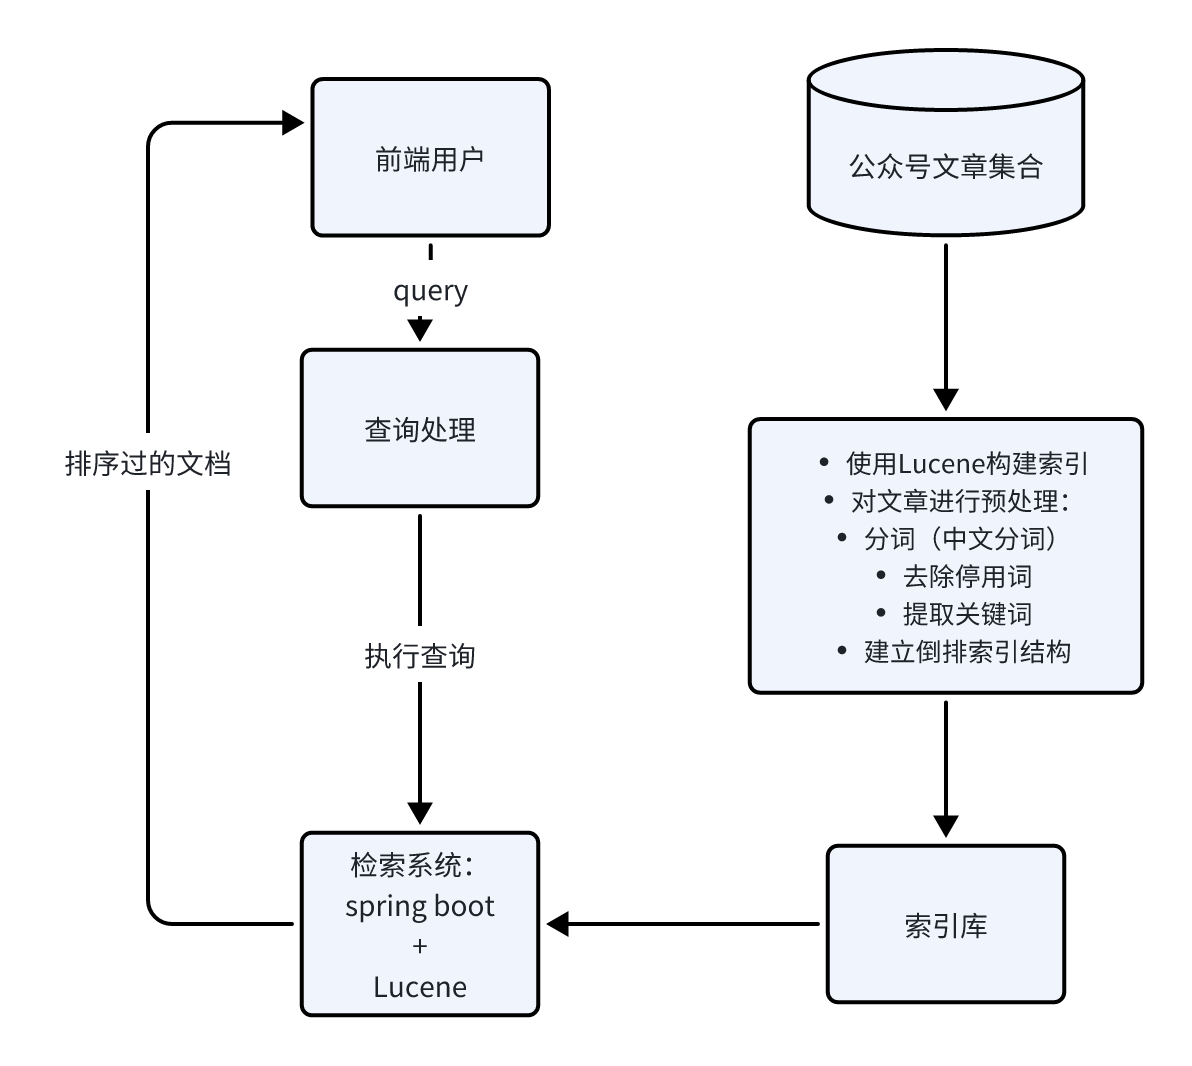
\includegraphics[width=0.7\textwidth]{figures/whiteboard_exported_image.png}
    \caption{IR系统基本框架构图(与Lucene框架对应)}
    \label{fig:ir_system}
\end{figure}

\subsubsection{爬虫技术的研究发展}
\songti\wuhao
网络爬虫技术,作为自动化获取互联网信息的核心手段,其重要性在数据驱动的时代背景下日益凸显。它使得大规模、系统性地收集网络资源成为可能,为后续的数据分析、信息检索和知识发现提供了基础。爬虫技术的发展历程,是伴随着互联网本身的演进和信息需求的不断深化而展开的。最初的网络爬虫主要执行简单的网页抓取任务,其功能相对单一,主要关注静态内容的获取\cite{ref5}。随着网络规模的急剧扩张和网页内容的动态化趋势,对爬虫技术的可扩展性、效率和智能性提出了更高要求。由此,分布式爬虫应运而生,通过多节点协作来提升抓取海量数据的能力\cite{ref3}。为解决数据时效性问题,增量式爬虫技术被提出,它能够智能地识别和更新已变化的内容,避免了全量重复抓取带来的资源浪费。同时,为了更精准地获取特定领域或主题的信息,聚焦式爬虫(Focused Crawler)通过引入主题相关性评估等策略,显著提高了采集信息的针对性和价值密度\cite{ref1}。此外,随着网站反爬虫机制的不断升级,如IP限制、User-Agent验证、动态加载、验证码等,爬虫技术也在持续演进,发展出更为复杂的应对策略和模拟技术,以保障数据获取的稳定性和成功率\cite{ref2}。在这一发展过程中,涌现了众多优秀的爬虫框架和相关技术,例如Python语言生态下的Scrapy、Beautiful Soup和Selenium等,它们极大地简化了爬虫的开发复杂度。本项目所选用的WebMagic,便是一款基于Java的高效、模块化爬虫框架。它借鉴并整合了现有爬虫技术的发展成果,提供了如页面下载、内容抽取、任务调度和数据持久化等核心组件,支持灵活的定制开发。选择WebMagic作为本系统的信息采集工具,正是基于其在处理结构化和非结构化数据方面的成熟能力,以及在保证采集效率和可靠性方面的良好表现,旨在为微信公众号文章这类特定信息源的自动化数据采集提供有力支持\cite{ref10}。

\subsubsection{目的与意义}
\songti\wuhao
本研究的核心目的在于设计并实现一个面向微信公众号的综合性信息系统。该系统旨在集成自动化文章采集、结构化数据存储、高性能全文检索、AI辅助内容分析(如智能摘要与关键词提取)以及便捷的标签化管理等多项功能。其直接目标是有效降低用户在面对海量微信公众号信息时的获取与管理成本,显著提升信息组织、查找的效率,并通过引入智能分析手段,深化对所采集内容的理解与利用价值。具体来说,本系统的研究目标包括:

\subsection{研究内容及方法}

\subsubsection{研究内容}
\songti\wuhao
本课题的主要研究内容包括以下几个方面:

\begin{enumerate}[label=\roman*., leftmargin=2em, itemsep=0pt, parsep=0pt]
\item 微信公众号平台自动化文章采集技术的设计与实现。
\item 公众号文章数据的解析、清洗及结构化存储方法研究。
\item 基于全文检索技术的文章检索模块构建与优化。
\item 基于中文信息处理技术的文章倒排索引、智能摘要及关键词提取研究。
\item 系统整体架构设计与前后端功能模块的实现。
\end{enumerate}

下图2、图3分别是前后端功能研究的不同系统模块划分。

\begin{figure}[htbp]
    \centering
    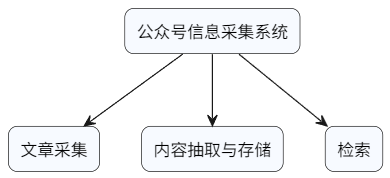
\includegraphics[width=0.8\textwidth]{图2:后端系统模块.png}
    \caption{后端系统模块划分}
    \label{fig:backend_modules}
\end{figure}

\begin{figure}[htbp]
    \centering
    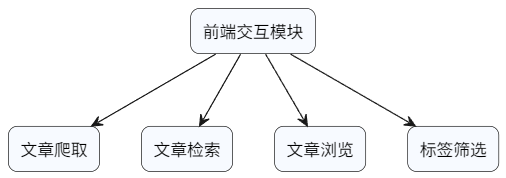
\includegraphics[width=0.8\textwidth]{图3-前端系统模块划分.png}
    \caption{前端系统模块划分}
    \label{fig:backend_modules}
\end{figure}

\subsubsection{研究方法}
\songti\wuhao
[此处添加研究方法内容]

\subsection{本课题的研究现状}
\songti\wuhao
[此处添加研究现状内容]

\subsection{本章小结}
\songti\wuhao
[此处添加本章小结内容]

\section{相关技术概述}

\subsection{系统架构简介}

\subsection{系统开发核心技术}

\subsubsection{Java语言与Spring Boot框架}

\subsubsection{Vue.js前端框架与UI组件库}

\subsubsection{MySQL关系型数据库}

\subsubsection{Maven项目构建工具}

\subsubsection{Apache Lucene全文检索引擎}

\subsection{微信公众号信息采集关键技术}

\subsubsection{WebMagic爬虫框架}

\subsection{全文检索与数据处理技术}

\subsubsection{Apache Lucene全文检索引擎}

\subsection{人工智能辅助技术应用}

\subsubsection{DeepSeek AI模型API}

\subsection{本章小结}

\section{系统设计与实现}

\subsection{系统总体架构与设计思想}

\subsubsection{后端总体架构设计与核心分层}

\subsection{数据库详细设计}

\subsubsection{逻辑结构设计}

\subsubsection{物理结构设计}

\subsection{核心功能模块详细设计与实现}

\subsubsection{爬虫模块设计与实现}

\subsubsection{搜索模块设计与实现}

\subsubsection{AI摘要模块设计与实现}

\subsubsection{标签系统模块设计与实现}

\subsection{核心模块接口设计}

\subsection{开发环境、依赖与工具}

\subsection{本章小结}

\section{系统测试与结果分析}

\subsection{测试方法与环境}

\subsubsection{测试方法}

\subsubsection{测试环境}

\subsection{主要功能模块测试用例与结果}

\subsubsection{文章爬取模块测试用例}

\subsubsection{文章搜索模块测试用例}

\subsubsection{AI增强功能测试用例}

\subsubsection{前端界面与用户体验测试用例}

\subsection{测试总结与质量评估}

\subsubsection{测试执行概况}

\subsubsection{发现的主要问题}

\subsubsection{测试结论}

\section{参考文献}

\begin{thebibliography}{99}
\songti\wuhao
\bibitem{ref1} 刘晓旭. 主题网络爬虫研究综述[J]. 电脑知识与技术, 2024, 20(8): 97-99.
\bibitem{ref2} 李志义. 网络爬虫的优化策略探略[J]. 现代情报, 2011, 31(10): 31-35.
\bibitem{ref3} 郭丙琴, 陈爱武. 分布式网络爬虫设计[J]. 湖南科技学院学报, 2017, 38(6): 21-22.
\bibitem{ref4} 周海晨. 基于爬虫与文本挖掘的"985"高校图书馆微信公众号的调研[D]. 安徽大学, 2017.
\bibitem{ref5} 霍英, 李小帆, 丘志敏. 基于大数据的网络数据采集研究与实践[J]. 软件工程, 2023, 26(4): 28-32.
\bibitem{ref6} Gormley C, Tong Z. Elasticsearch: The Definitive Guide[M]. O'Reilly Media, 2015.
\bibitem{ref7} 杨晓丰. "双一流"高校图书馆微信公众平台运营量化研究[J]. 图书馆学刊, 2021, 43(1): 49-53.
\bibitem{ref8} 肖文娟, 王加胜. 基于Vue和Spring Boot的校园记录管理Web App的设计与实现[J]. 计算机应用与软件, 2020, 37(4): 25-30.
\bibitem{ref9} Zmaranda D R, Moisi C I, Győrödi C A, et al. An Analysis of the Performance and Configuration Features of MySQL Document Store and Elasticsearch as an Alternative Backend in a Data Replication Solution[J]. Applied Sciences, 2021, 11(24): 11590.
\bibitem{ref10} Liu Q, Yahyapour R, Liu H, et al. A novel combining method of dynamic and static web crawler with parallel computing[J]. Multimedia Tools and Applications, 2024, 83(21): 60343-60364.
\end{thebibliography}

\end{document}